\chapter{Graphics Adapter Background}
\label{BACKGROUND}

To begin this chapter, PC graphics adapter history is explored. The history
concludes with an overview of VGA as all earlier specifications are now
considered obsolete. The primary graphics adapter in a PC must be VGA compatible
in order for the system to boot. The main functional components of a VGA adapter
are then introduced followed by a brief explanation of these components.

OpenVGA is not the first open graphics adapter project either so other
similar projects are investigated. Completing this chapter, the similarities and
differences with these other projects, relative to OpenVGA, are examined. Amongst
others, the capable and prominent, though complex and expensive, OpenGraphics
adapter is covered here.


\begin{figure}[h!]
\begin{center}
\includegraphics[width=\linewidth]{images/vga_overview.pdf}
% \includegraphics[width=\linewidth]{images/ati_rage.eps}
% convert -resize 1024 ati_rage.jpeg eps3:ati_rage.eps
\caption[ATi Rage graphics adpater]{ATi Rage graphics adapter with the
significant components identified.}
\end{center}
\label{INTRO_ATi_Rage}
\end{figure}


\section{PC Graphics Adapter History}
The original IBM PC featured a Monochrome Display Adapter (\gls{mda})~\cite{VGA_Programmers}. The MDA
only had a very small local memory due to the high cost of DRAMs. This memory
only stored \gls{ascii} (American Standard Code for Information
Interchange, see Figure~\ref{INTRO_ASCII}) and attribute data for
several screenfuls of text (80 columns and 25 rows of ASCII characters). The MDA
had dedicated hardware which converted ASCII characters from text-buffer into
pixel values during display redraw periods. The pixel values were transmitted to
a monochrome \gls{crt} monitor for
display.

The original IBM PC was produced from readily available parts and was reverse
engineered by other companies to produce numerous compatible versions. This means
that the MDA had to be reverse engineered. Derivatives were produced that had
more features and were backwards compatible, like the Hercules graphics adapter
(sometimes called HGA).

The original IBM PC was the first in a line of computers, with future models
having different hardware, including changes to the display adapters. The later
graphics adapter standards: CGA, MCGA, EGA, VGA, 8514, XGA, and TIGA; all
followed MDA. These later adapters were reverse engineered and cloned as well,
though the display adapter standards after VGA never gained widespread
use~\cite{VGA_Programmers}.

VGA was extended by many manufacturers, increasing framebuffer sizes, numbers of
colours, higher resolution modes, and hardware acceleration for 2D and 3D
functions. The umbrella term for all of these adapters was Super
VGA, or \gls{svga}. Every time a
different manufacturer produced a VGA compatible display adapter, they
essentially had to start from scratch, reimplementing VGA and adding their own
extensions. Some of these companies were: Oak, Advance, Genoa, NCR, Integrated
Info Tech, Tseng Labs, Weitek, Trident, Western Digital, Video7, VIA, SiS, Chips
and Technologies, Cirrus Logic, ATI, Nvidia, Intel, S3, and 3DFX.


\section{The Original IBM VGA}
The major components of a VGA-compatible graphics adapter are shown in
Figure~\ref{INTRO_ATi_Rage}. These components being: a VGA IC\footnote{The
earlier VGA adapters typically used separate ICs for the RAM DAC and the VGA, but
with this adapter, the functionality is combined into the main IC. Additionally,
this adapter contains hardware support for 3D graphics acceleration.}, some
memory for a framebuffer, a ROM containing the VGA BIOS, connector for
communicating with the host, connector(s) for attaching a display device, and
some power supply circuitry.


\subsection{The Video Graphics Array}
Before VGA, the graphics adapter's functional components were contained within
multiple ICs. VGA was IBM's first adapter which contained the majority of the
logic functionality within a single IC. The functions that were combined
into one ASIC were:

\begin{itemize}
  \item CRT controller
  \item Attribtue controller
  \item Sequencer
  \item Pixel data serialiser
  \item Graphics controller
  \item Miscellaneous control registers
  \item ASCII text to pixel converter
  \item Bus interface logic
  \item Memory controller
\end{itemize}


The CRT Controller (\gls{crtc})
generates the timing signals necessary to display an image on a VGA or DVI
connected monitor. Images are sent to a monitor as a stream of pixels, scanning
from left to right, and from top to bottom. The CRTC generates the signals which
synchronise the pixel-stream being sent. These are the horizontal
synchronisation (\gls{hsync}) signal that indicates the end of the current horizontal line, and the
vertical synchronisation (\gls{vsync}) signal that marks the end of the current screen (see
Figure~\ref{INTRO_CRT_Redraw} for more detail).

\begin{figure}[h!]
\begin{center}
\includegraphics[width=0.9\linewidth]{images/crt_redraw.pdf}
% \includegraphics[width=0.9\linewidth]{images/crt_redraw.eps}
\end{center}
\caption[VGA display redraw timing and signals]{VGA display redraw timing and
signals. (Image from~\cite{knutsson:fbg}.)}
\label{INTRO_CRT_Redraw}
\end{figure}

Early VGA adapters, like their predecessors, had a very limited quantity of
framebuffer memory to store the image to be displayed, due to the price of DRAM
ICs. Rather than store every colour as \gls{rgb} (Red Green Blue) components, the colours were stored as indices into
a colour palette. The palette contained the corresponding colour for a given
index, and the palette only contained indices for a subset of available colours.
This technique allowed the use of smaller framebuffers.

In monochrome modes, for example, one bit encodes the colour, so it can only be
one of two values. VGA supported 1-bit, 2-bit, 4-bit, and 8-bit colour modes. The
attribute controller was responsible for converting these colour indices into the
full 24-bit RGB colour format that the video DAC then converts to VGA compatible
analogue signals.

The attribute controller contains two colour look-up tables, or palettes, and
these are typically daisy-chained, the output of the first becoming the input to
the second (except in 8-bit, packed-pixel modes, where the first table was not
used). The first palette takes as input a 4-bit value and generates a 6-bit
value. This 6-bit value is combined with some additional register values, and is
used to generate the an 8-bit index into the second table. This 8-bit index into
the second palette retrieves an 18-bit output RGB value, 6-bits per colour
component, and is then combined with additional attribute controller registers to
extend it to the final 24-bit RGB format.

The attribute controller has other programmer accessible features too, it can
also mask pixels from any of the four bit-planes, depending on the video mode, can
enable pixel blinking, and can pan the display horizontally, which works in both
graphics and alphanumeric modes.

To set a single pixel, in the 4-bit colour mode for example, a single bit from
each of the four bit-planes (see the display memory explanation in
Section~\ref{VGA_Display_Memory}) may need to be modified, therefore each of the
four DRAMs needs to be accessed. To improve performance with these operations,
the graphics controller allows various programmer-set, bitwise operations and
shifts to be performed on the incoming data and combines these modified values
with the data stored in the bit-planes. Afterwards, the modified values are
written back to the DRAMs, and these operations are pipelined to achieve high
performance.

All of the timing signals required for the VGA are controlled by the sequencer,
and often generated from a single off-chip oscillator. The sequencer generated
dot-clock and character-clock signals control the timing for nearly all of the
VGA, with the exception of the external bus clock signal. One last feature of the
sequencer allows the bit-plane to be enabled or disabled too.

Pixel colour-values are not stored within the display memory when the VGA is
operating in alphanumeric modes. Only ASCII-encoded text along with its
corresponding attributes (see Figure~\ref{INTRO_ASCII} to see how ASCII
alphanumeric fonts were stored as bit-masks), and a font bit-mask, are stored in
the display memory. The attributes values for each ASCII character are foreground
and background text colour, and optionally a value that causes that particular
character to blink\footnote{Character blinking is achieved by periodically
swapping foreground and background colour as the character is decoded into
pixels.}. These alphanumeric modes were created since the memory storage
requirements are far lower than graphics modes where every pixel is addressable.
In the standard 80 column, 25 row, alphanumeric mode (from now on referred to as
80x25 text-mode), only requires 4 kB of DRAM. Due to the low memory requirements
of alphanumeric modes, up to eight ``pages'' were supported, and could be
dynamically exchanged by modifying user programmable registers.

\begin{figure}[h!]
\begin{center}
\includegraphics[width=\linewidth]{images/ascii.png}
\caption[ASCII and extended-ASCII character set]{ASCII and extended-ASCII
character sets, and an example pixel representation.}
\label{INTRO_ASCII}
\end{center}
\end{figure}

VGA, and all earlier display adapters produced by IBM, includes dedicated
hardware for performing ASCII-character to pixel conversion, since it needs to
operate continuously while in alphanumeric modes. ASCII text is retrieved from
the framebuffer at the rate of the character clock, and converted to pixel data
at the rate of the dot-clock, which is 25.175 MHz in the default VGA 80x25
text-mode. The default VGA text-mode resolution is 640x400 pixels, with a redraw
rate of 60 Hz, and for the system's \gls{x86} processor (the generic name for the Intel
8086 CPU architecture and derivatives) to produce pixel values at this rate would have been difficult
in 1987 .

\begin{table}[h!]
\begin{center}
\begin{tabular}{c | c l}
Port & Direction & Register Description \\
\hline
3B4h & R/W & CRTC Controller Address Register \\
3B5h & R/W & CRTC Controller Data Register \\
3BAh & Read & Input Status $\#1$ Register \\
3BAh & Write & Feature Control Register \\
3C0h & R/W & Attribute Address/Data Register \\
3C1h & R/W & Attribute Data Read Register \\
3C2h & Read & Input Status $\#0$ Register \\
3C2h & Write & Miscellaneous Output Register \\
3C4h & R/W & Sequencer Address Register \\
3C5h & R/W & Sequencer Data Register \\
3C7h & Read & DAC State Register \\
3C7h & Write & DAC Address Read Mode Register \\
3C8h & R/W & DAC Address Write Mode Register \\
3C9h & R/W & DAC Data Register \\
3CAh & Read & Feature Control Register \\
3CCh & Read & Miscellaneous Output Register \\
3CEh & R/W & Graphics Controller Address Register \\
3CFh & R/W & Graphics Controller Data Register \\
3D4h & R/W & CRTC Controller Address Register \\
3D5h & R/W & CRTC Controller Data Register \\
3DAh & Read & Input Status $\#1$ Register \\
3DAh & Write & Feature Control Register \\
\end{tabular}
\end{center}
\caption[VGA I/O Ports]{VGA I/O Ports.}
\label{PCI_VGA_Port_Table}
\end{table}

All of the control registers of VGA were mapped to x86 I/O ports and these are
listed in Table~\ref{PCI_VGA_Port_Table}. For a device to be VGA-compatible,
these control registers have to be emulated. These registers were extended by
SVGA to allow more video modes, but these were not standardised between
manufacturers. Subsequently, directly programming SVGA registers is complicated,
but there are books which detail the programming of the more popular SVGA
graphics cards~\cite{SVGA_Book, VGA_Programmers}.


\subsection{Video DAC}
The video DAC converts 24-bit, RGB-encoded, colour values into the analogue
signals required to drive a VGA display. The video DAC was originally a
separate IC~\cite{VGA_Programmers, SVGA_Book} though modern graphics adapters
can include them within the main ASIC (see Figure~\ref{INTRO_ATi_Rage}). The
digital encoding consists of three 8-bit fields, representing each RGB colour
component, and the DAC produces analogue values which range in magnitude between
0.7 and 1.4 V.


\subsection{VGA BIOS}
Each VGA device requires a VGA Basic Input/Output System (\gls{bios}) \gls{rom}. This is a collection of
routines for performing video functions. These routines are accessed on an x86 PC
architecture by using software interrupts (using the instruction `int 10h',
register values are used as the arguments)~\cite{VGA_Programmers, SVGA_Book}, and
are typically written in just 16-bit, Intel 8086, assembly code.

The VGA BIOS contains routines for changing modes, setting pixels, cursor
positioning, and many others. These routines are required for VGA compatibility.
A separate ROM IC containing this code is usually present on a VGA board, as
shown in Figure~\ref{INTRO_ATi_Rage}. A free and open source implementation of
the VGA BIOS is available, and this is included within the OpenVGA project since
it provides all the required functionality, complete with a VESA BIOS Extensions
(VBE) implementation.


\subsection{Display Memory}
\label{VGA_Display_Memory}
The original IBM VGA had display memory that consisted of four 8-bit DRAMs, and
each DRAM contained the data for one of the four bit-planes (except in
packed-pixel modes, where the memory was not arranged as planes). The total
quantity of display memory on original VGA adapters was typically 256 kB, though
versions were available with only 64 kB or 128 kB of DRAM and could not support
all video modes. The portion of display memory which is involved with redrawing
the screen in the current mode is also called the framebuffer, as it stores
(buffers) the data for the current frame.

A VGA display adapter has graphics modes, which are also called ``all points
addressable'' modes, in which every pixel is mapped to a location in memory (or
multiple ``bit-planes'' in some VGA modes). For the 640x480 resolution graphics
mode, the maximum resolution officially supported by the original IBM VGA, there
are 307,200 pixels, each can be set individually. Some graphics modes support
multiple pages of image data. These can be exchanged, typically during the
vertical-synchronisation period, to achieve a smooth animation effect.


\section{Non-VGA Graphics Adapters}
Graphics adapters have been developed and produced that are designed to be
installed and used alongside a VGA adapter within a PC. Prominent examples are a
couple of the 3D graphics accelerators produced in the 1990s, the PowerVR Series
1, and 3DFX Voodoo Graphics (later referred to as Voodoo 1) and Voodoo 2. The
primary graphics adapter, typically a SVGA, is used for all 2D modes, like those
commonly used by OS Graphical User Interfaces (\gls{gui}s). Once a 3D application is started,
like a computer game, the 3D graphics accelerator is activated and is used to
redraw the display instead.

The PowerVR and Voodoo 1 \& 2 adapters used a pass-through architecture, where
the primary graphics adapter had its output redirected to the 3D accelerator, in
a daisy-chain configuration. This was achieved with a short ``loopback'' cable
routed from the primary adapter to the input port of the secondary adapter. The
output of the secondary adapter was connected to the display device, typically a
SVGA CRT monitor.


\section{Related Projects}
There exists several other graphics adapter projects, and a brief overview of
these is given. The most extensive of these is the Open Graphics Project, with
aims to produce both FPGA and ASIC graphics adapters, and including support for
multiple operating systems. Also planned is 3D acceleration, including support
for \gls{opengl}~\cite{OpenGL}, an open-specification 3D graphics library.


\subsection{Open Graphics Project}

\begin{figure}[h!]
\begin{center}
\includegraphics[width=\linewidth]{images/ogd1_showcase.jpeg}
\end{center}
\caption[OpenGraphics OGD1]{OpenGraphics OGD1 PCB and components. (Image
from~\cite{OpenGraphics}.)}
\label{INTRO_OGD1}
\end{figure}

Open Graphics Project\footnote{For more information see http://opengraphics.org/}
is a prominent open-source VGA project, which aims to develop a VGA compatible
display adapter with hardware 3D acceleration support, and OpenGL drivers.
Development is currently using an FPGA-based board, called OGD1 (See
Figure~\ref{INTRO_OGD1}), but the project's stated goal is to raise enough money
to have an ASIC fabricated.

OpenGraphics has an impressive feature list, allowing for a very capable graphics
adapter, and is significantly more complex than what was planned for OpenVGA, but
the cost of the development boards is around 1000 USD. Their plan is to emulate
VGA using a soft processor core. The OGP processor core is a 32-bit RISC design,
and the architecture is similar to a MIPS processor~\cite{OpenGraphics}.

The OpenGraphics source code is freely available and licensed under the GPL, but
all contributions back to the project require copyright be assigned to Traversal
Technologies Incorporated so they can dual-license the code to sell commercial
versions of it.

At the time of writing this, the development of OGP has reached the point where
they have OGD1 running as a simple non-VGA framebuffer device, and now can run
code on their soft-processor core too.


\subsection{Project VGA}

% \begin{figure}[h!]
% \begin{center}
% \includegraphics[width=\linewidth]{images/project_vga.eps}
% \end{center}
% \caption[Project VGA Photograph]{Project VGA promotional photograph.
% \textit{Image obtained from http://wacco.mveas.com/}}
% \label{INTRO_ProjectVGA}
% \end{figure}

This project has stated aims similar to OpenVGA, it aims to be low-cost, simple,
VGA compatible, open-source graphics adapter (see http://wacco.mveas.com/).
Unfortunately though, the status of this project does not appear to have been
updated since 28/02/08 .


\subsection{Manticore}
The goal of this project was to develop a non-VGA, 3D graphics accelerator, and
once this stage was complete, add 2D support to it. The project uses an older model
Altera FPGA and does not seem to have been updated in the last three years.
